\documentclass[12pt,letterpaper]{report}
\usepackage[margin=1in]{geometry}
\usepackage{titlesec}
\usepackage{amsmath}
\usepackage{amssymb}
\usepackage[colorlinks=true,urlcolor=black,linkcolor=black]{hyperref}
\usepackage{graphicx}
\usepackage{textcomp}
\graphicspath{ {./images/} }
% extra packages you need

\titleformat{\chapter}{\bf\huge}{\thechapter}{20pt}{\huge\vspace{-.5em}}

\begin{document}

\title{\begin{figure}[htb]
\begin{center}

\includegraphics[width=8cm]{univ_logo}
\end{center}
\end{figure}SOEN 6011 : SOFTWARE ENGINEERING PROCESSES\\[.5em]
SUMMER 2022\\\vspace*{0.9in}
\begin{Large}
\textbf{ETERNITY} 
\end{Large}
\vspace*{0.9in}
\begin{Large}
\textbf{\\PROBLEM - 4} 
\\Error Handling, Debugger  \& Quality Attributes\\ 
\small{https://github.com/PrathikaSuvarna/ScientificCalculator}
\end{Large}}
\author{By Prathika Anup Suvarna (40156790)}
\maketitle 
\pagenumbering{roman}
\setcounter{page}{0}

\tableofcontents

\chapter{Error Handling}
\pagenumbering{arabic}
Error handler in a program works when there is an unexpected error condition in the program.
In my calculator, that implements the standard deviation function, if the user clicks on the $\sigma$ button without giving any input or tries to give a character as an input,the program
will notify the user by sending an error message.
The error handling is mainly done using the try..catch method.

{\let\clearpage\relax \chapter{Graphical User Interface}}
I have implemented a graphical user interface for my calculator to calculate the standard deviation of an array of numbers.
\\\\
\begin{center}
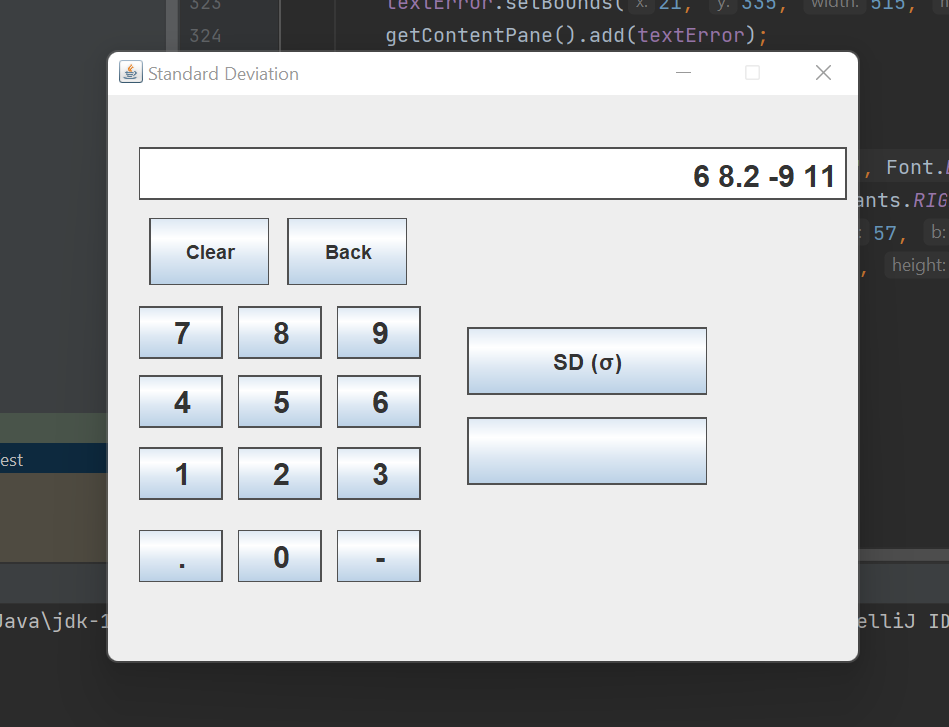
\includegraphics[width=8cm]{ui}
\end{center}

\chapter{Debugger}

\section{Description}
Debugging is a method to detect various errors in the source code and removing all the errors from the software code that is causing problem in the implementation of the code.
In order to debug the source code, I have used the in-built Intellij debugger where we can add suitable breakpoints and run the program in debugging mode. Intellij debugger gives us the various potential functions to help in running the code step by step and detect the potential bugs. 

\begin{center}
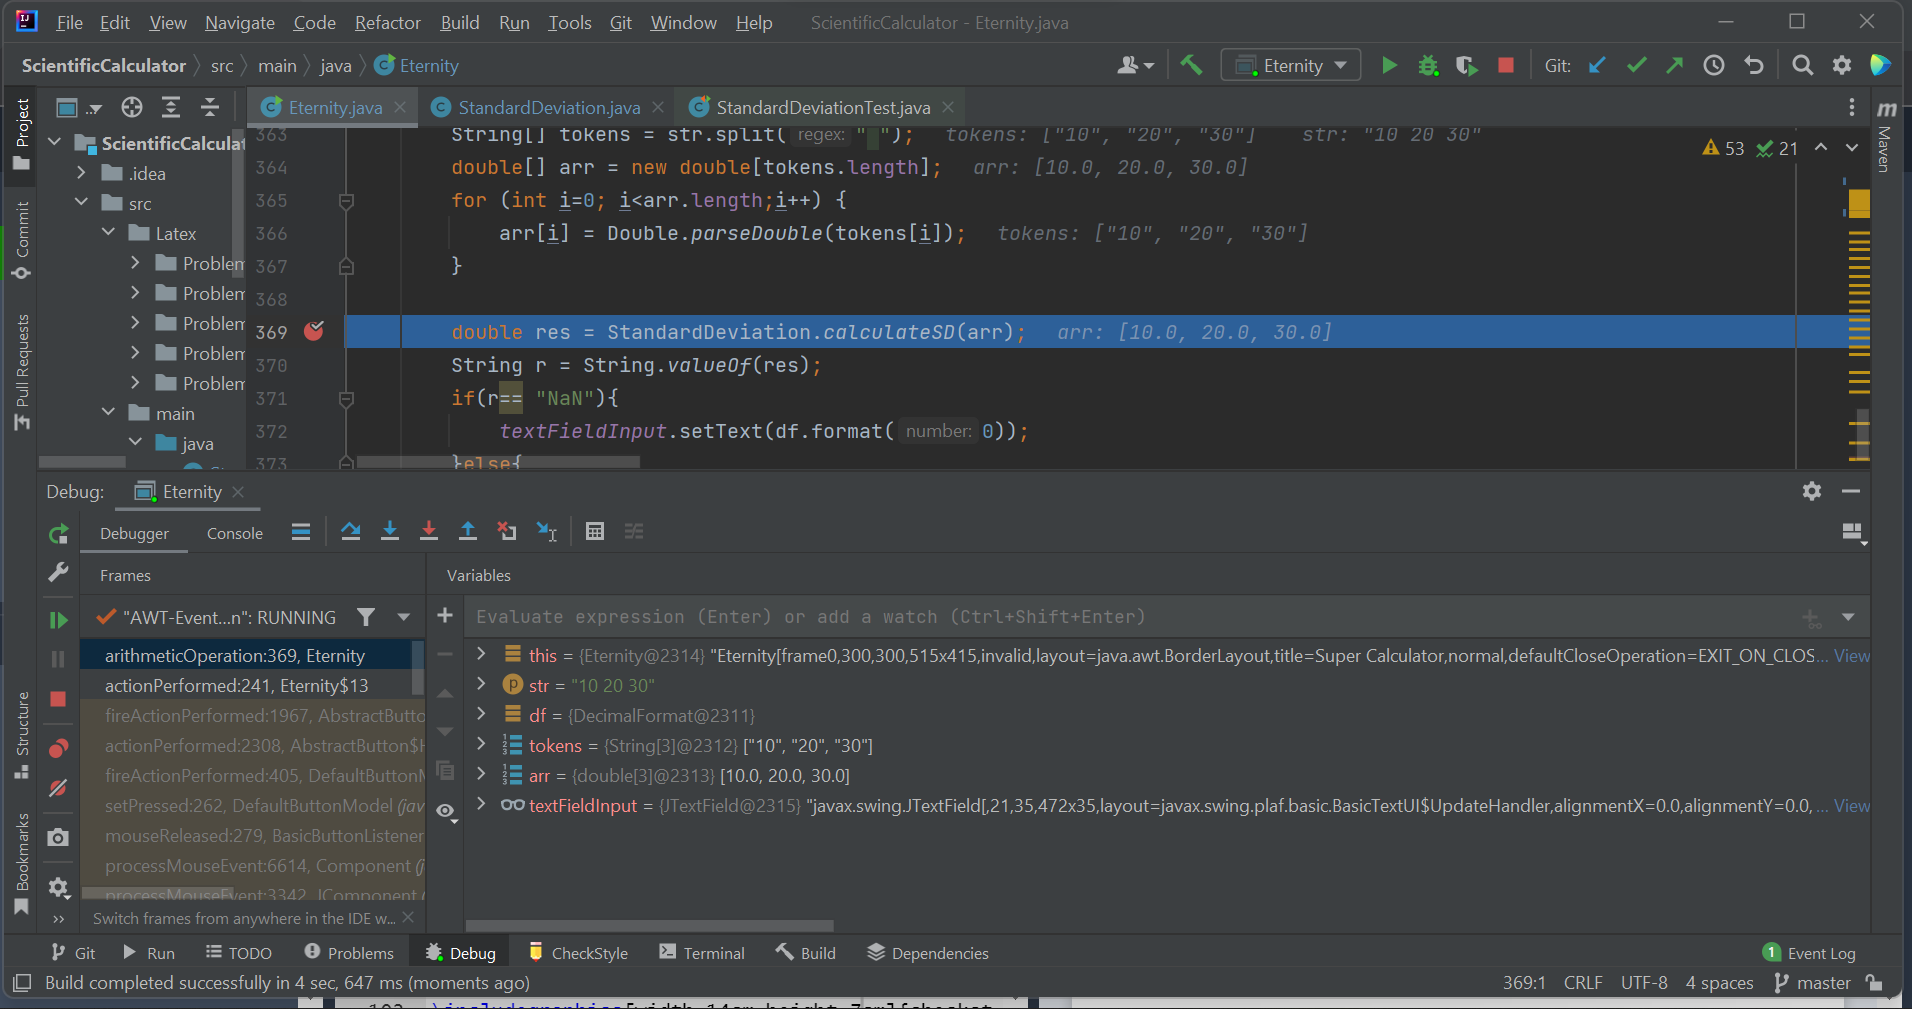
\includegraphics[width=14cm,height=7cm]{debug}
\end{center}

\section{Advantages}

\begin{itemize}
    \item There is an option of event based breakpoints.
    \item We can modify the program by using debugger to make it more efficient and make it free from errors.
    \item The variables value can be changed at any time while debugging the code.

\end{itemize}

\section{Disadvantages}
\begin{itemize}
    \item Some programs have multi-threading, which makes it more complicated to control the program.
    \item Debugging can be time consuming as it is testing each line of code.
\end{itemize}

{\let\clearpage\relax \chapter{Quality Attributes for the source code }}


\section{Correctness}
My source code for the standard deviation function is tested with all the possible values including positives, negatives, decimals and compared with 2-3 online calculators. The results are found to be accurate and precise. 

\section{Maintainablity}
The program is split into several functions which make it more easier to maintain the source code. In addition to this, necessary comments and javadocs have been added to make it more maintainable.

\section{Robustness}
The program is handling various errors and exceptions which can occur while users enter an incorrect input. 

\section{Time-efficient}
Suitable breakpoints have been chosen for debugging the code which results in time-efficiency.

\section{Usability}
The program is user-friendly as we have used the "Graphical user-interface" for accepting inputs from the user.


\chapter{Checkstyle}

\section{Description}
Checkstyle is a plug-in/tool for IntelliJ that i installed and ran to automatically check the Java source code  against a configurable set of rules. It helps the programmers to write Java code that sticks and follows a coding standard. I have made some changes after checking the quality of my code
using checkstyle.
\\\\
\begin{center}
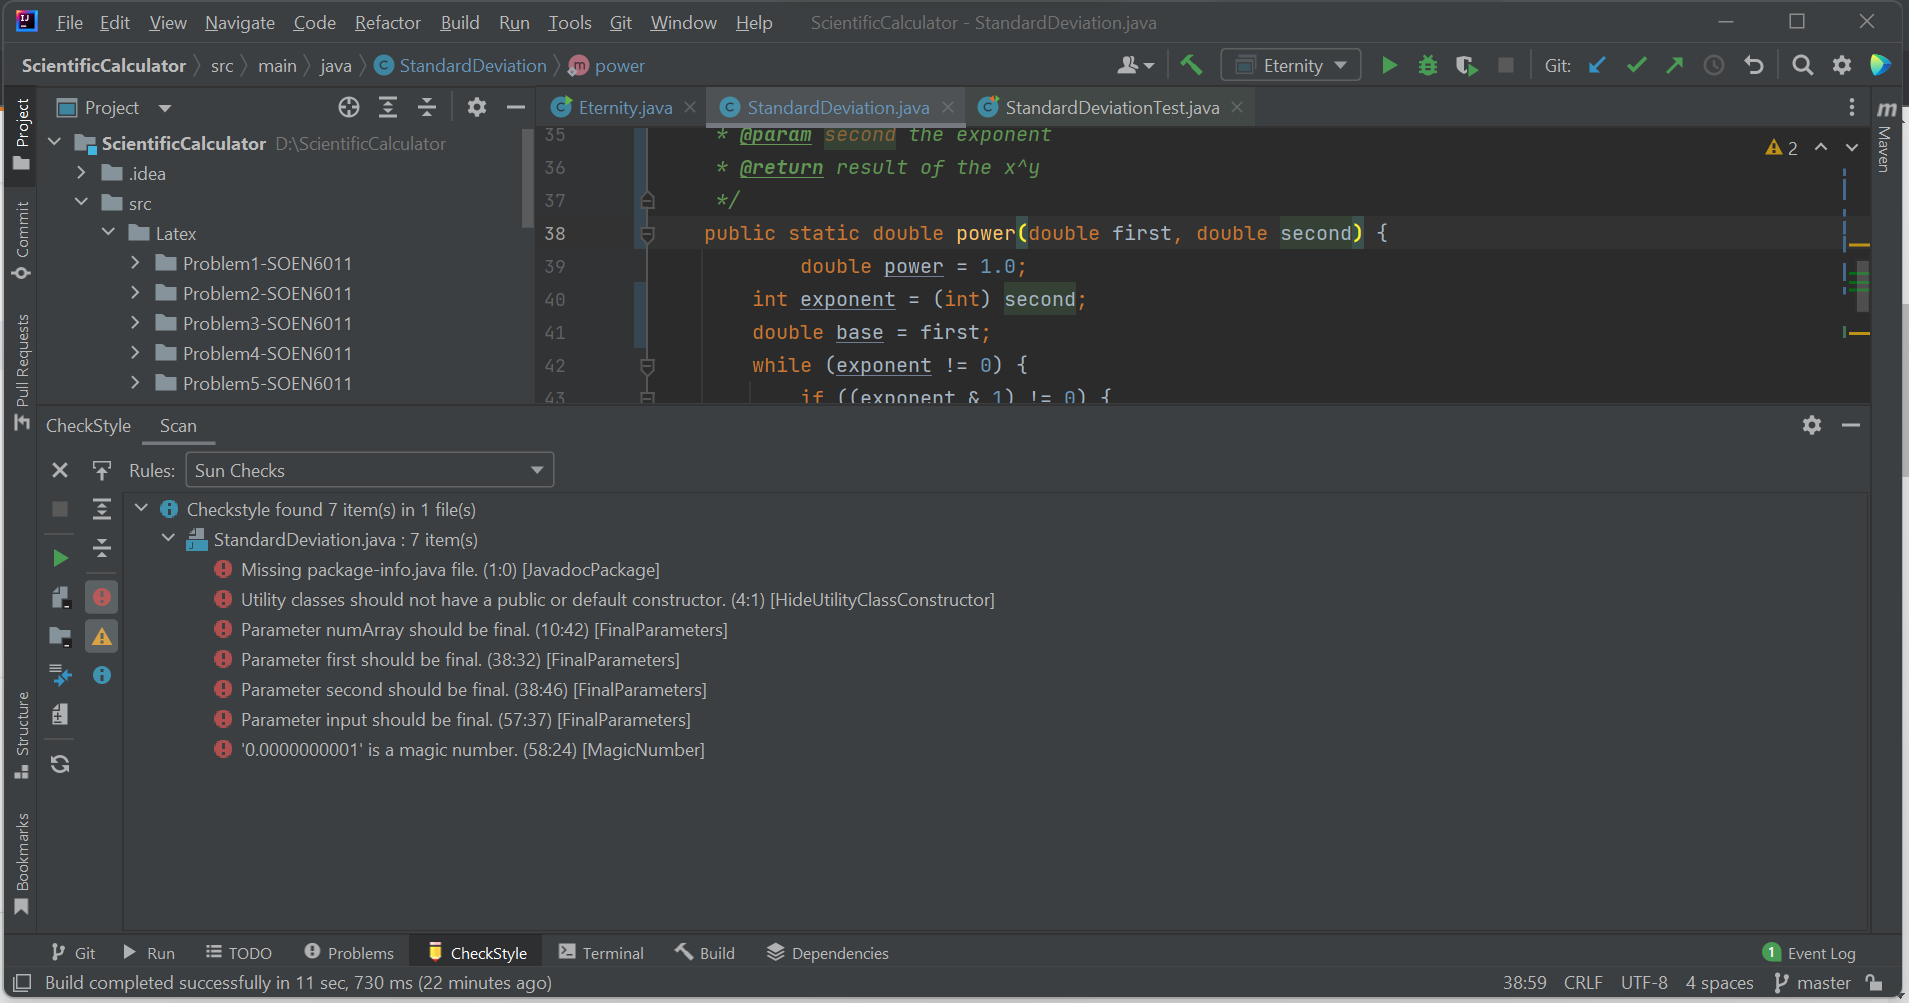
\includegraphics[width=14cm,height=7cm]{checkstyle}
\end{center}

\section{Advantages}

\begin{itemize}
    \item Checkstyle can check many things in the Java source code. From checking the code layout to the code formatting, it is handling everything.
    \item It has ability to create own rules for handling Java source code. Also, it can support any coding standard.
    \item Checkstyle is portable as it is easy to switch between different IDEs. In addition to this, it can find class design problems and method design problems.

\end{itemize}

\section{Disadvantages}
\begin{itemize}
    \item It does not support any auto correct features to check any invalid coding standards.
    \item All the identifiers and keywords should be written in ASCII format only.
    \item Checkstyle tool is used only to check the format of the code and not the correctness of the code.
\end{itemize}









\begin{thebibliography}{9}
\addcontentsline{toc}{chapter}{Bibliography}
\bibitem{Debugger} 
Debugger
\\\texttt{https://www.techtarget.com/searchsoftwarequality/definition/debugging}

\bibitem{Checkstyle}
Checkstyle
\\\texttt{https://checkstyle.sourceforge.io/}



\end{thebibliography}



\end{document}